\section{Metadades}\label{sec:metadata}

Les metadades són el conjunt d'etiquetes presents a qualsevol registre que contenen informació sobre aquest.
Els autors, la descripció del recurs, la data de pujada, el departament responsable, el tipus de document, o més, es troben inclosos. \\

\noindent
En el nostre cas, a \gls{UPCommons}, aquestes utilitzen el format \gls{DSpace} Intermediate Metadata, \gls{DIM}, que es basa en fer sservir el format Dublin Core incorporant un qualificador, amb la finalitat d'afinar la informació que inclous.
L'estructura és la següent:

\begin{center}
    \textit{schema.element.qualifier} \\
\end{center}

\noindent
Per exemple, l'autor principal d'un recurs s'identificaria com:

\begin{center}
    \text{dc.contributor.author} \\
\end{center}

\begin{figure}[htbp]
    \centerline{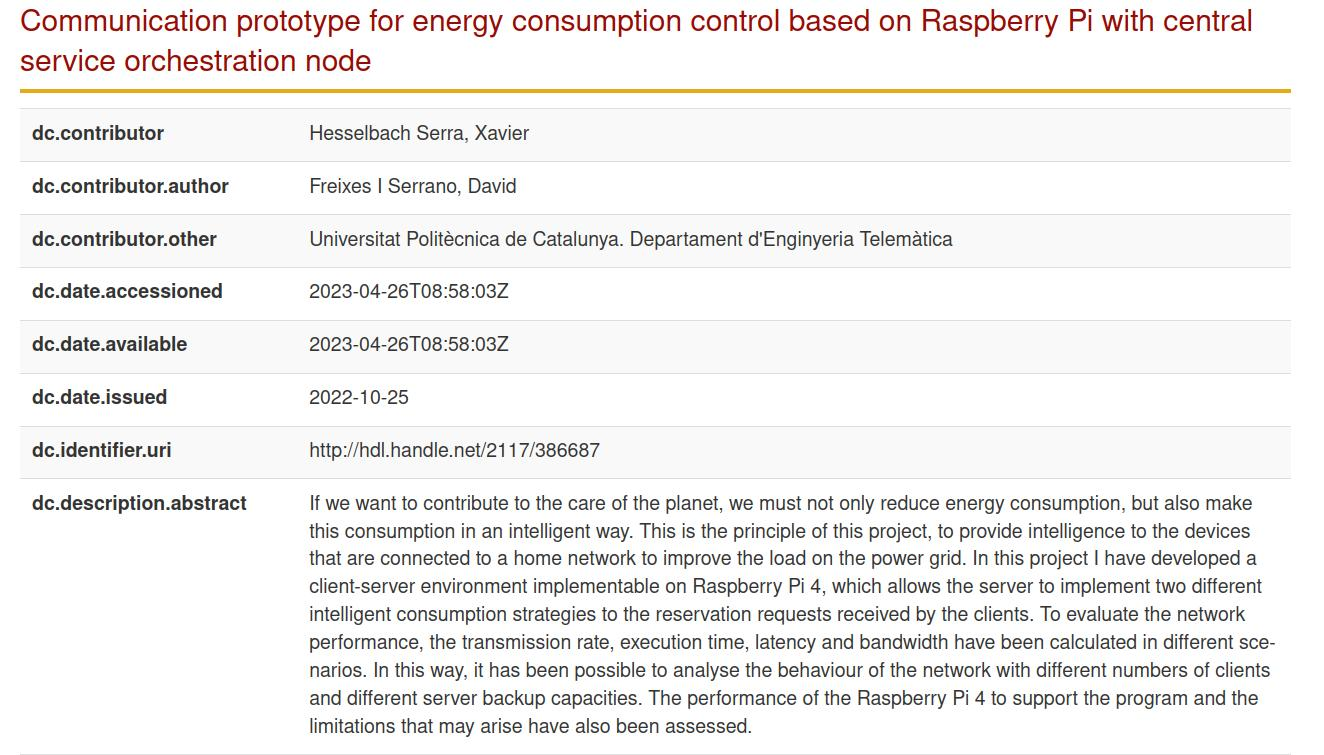
\includegraphics[width=0.8\textwidth]{figures/metadata-example}}
    \captionsetup{justification=centering}
    \caption{Llista parcial de les metadades del recurs}\label{fig:metadata-example}
    \source{\url{http://hdl.handle.net/2117/386687}}
\end{figure}



\noindent
Per cada metadada, s'assignen els següent valors:

\begin{itemize}
    \item \textbf{value}: Valor de la metadada.
    \item \textbf{language}: Idioma. És habitual trobar-lo a les descripcions / resums dels registres, encara que a vegades no està ben introduït.
    \item \textbf{authority}: Codi que relaciona la metadada amb un sistema d'autoritats que permet obtenir més dades.
    \item \textbf{qualifier}: Un nivell de confiança associat a l'autoritat.
\end{itemize}

\begin{figure}[htbp]
    \centerline{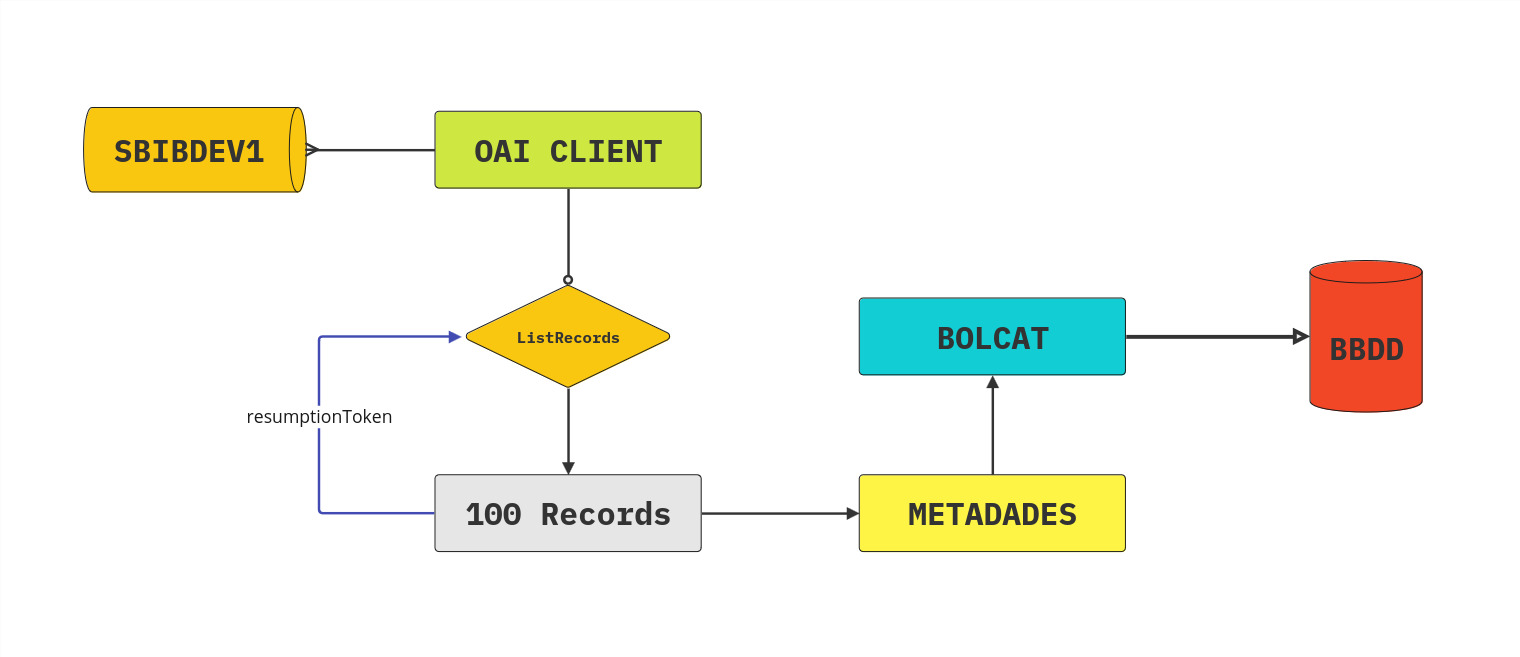
\includegraphics[width=1.2\textwidth]{figures/metadata-processing}}
    \captionsetup{justification=centering}
    \caption{Disseny tècnic del processament de les metadades.}\label{fig:log-analysis}
    \source{Elaboració pròpia.}
\end{figure}
